\documentclass[journal]{IEEEtran}

\usepackage{amsmath,amssymb}
\usepackage{graphicx}
\usepackage{booktabs}
\usepackage{siunitx}
\usepackage{url}

\graphicspath{{figures/}}
\newcommand{\Cuk}{\'{C}uk}
\newcommand{\TSRLS}{TS-D-RLS}
\newcommand{\TSKF}{TS-SLTVKE}

\title{Supervised Covariance Reset Resolves the Tracking--Confidence
Tradeoff in Topology-Synchronous Capacitor Health Estimation}

\author{Anonymous Author(s)}

\begin{document}
\maketitle

\begin{abstract}
Topology-synchronous decoupled observations identify the capacitance and
equivalent series resistance (ESR) of the \Cuk{} energy-transfer capacitor
from normal switching, but their two published realizations trade point
tracking against confidence calibration: a direction-decoupled recursive
least-squares (RLS) estimator tracks and recovers quickly with
uncalibrated intervals, whereas the Kalman realization reports calibrated
intervals but freezes after abrupt health changes because its innovation
gate then rejects every row. This letter adds a per-direction two-sided
CUSUM supervisor that consumes both accepted and gate-rejected normalized
innovations and, on alarm, resets that direction's covariance to its
initialization value. On identical simulated observation streams over a
54-case blind-style matrix at two noise levels, the supervised estimator
matches its Kalman parent in steady state (joint 95\% coverage
96.9\%/93.4\%; false-alarm cost at most 0.05 percentage points), recovers
from abrupt $-20\%$ capacitance and $2\times$ ESR steps in 2--3 switching
cycles instead of 527--868 (RLS) or never (Kalman), and reduces the
hardest 0.1-s ramp capacitance tracking error below both parents, at
about six extra operations per row. Results are simulation-only; the
components are classical, and the contribution is the gated
topology-synchronous construction that removes the documented tradeoff.
\end{abstract}

\begin{IEEEkeywords}
Capacitor condition monitoring, \Cuk{} converter, change detection,
Kalman filters, recursive least squares.
\end{IEEEkeywords}

\section{Introduction}
Capacitance loss and ESR growth are established degradation precursors in
power converters \cite{wang2014reliability,zhao2021overview}, and joint
C--ESR estimation from converter waveforms is a mature line of work
\cite{yao2015buck,hasegawa2018dclink}. For the \Cuk{} energy-transfer
capacitor, the companion paper \cite{companion2026} constructs
direction-decoupled, topology-synchronous observations---an ESR-dominant
switching-edge row and a capacitance-dominant safe-window charge row---and
evaluates two realizations on a common gated observation stream: \TSRLS{},
a direction-specific scalar RLS pair, and \TSKF{}, a structured Kalman
estimator with normalized-innovation-squared (NIS) gating.

That evaluation left a documented tradeoff. \TSRLS{} delivered the better
tracking, convergence, and abrupt-step recovery, but its auxiliary
intervals covered only 13\% jointly; \TSKF{} delivered calibrated
intervals (88.9\%) but failed to recover from abrupt health steps: once
the parameter jumps, every innovation exceeds the NIS gate, the update is
rejected, the covariance stays small, and the estimate freezes at the
stale value. The companion paper retained this failure as a negative
result and named an adaptive change detector as future work.

This letter closes that loop. The proposed construction leaves the Kalman
realization untouched in steady state and adds a supervisor built from
classical components---Page's CUSUM statistic \cite{page1954cusum} and
covariance resetting from adaptive filtering practice
\cite{mehra1970adaptive,willsky1976survey,gustafsson2000adaptive,barshalom2001estimation}.
The mechanism observation is that the gate-rejected innovations, which the
point update discards, carry exactly the sustained same-sign evidence of a
parameter change; supervising them recovers RLS-class adaptation without
giving up the Kalman covariance readout. Neither component is claimed as
new; the contribution is their direction-specific use on gated
topology-synchronous rows and the demonstrated resolution of the
tracking--confidence tradeoff.

\section{Supervised-Reset Construction}
Each accepted observation row is scalar in one health direction
$j\in\{C,R\}$ \cite{companion2026}: $z_{j,k}=h_{j,k}\theta_j+\nu_{j,k}$,
with $\theta_C=\bar\alpha$ (normalized inverse capacitance) and
$\theta_R=r_C$. The Kalman kernel per direction is the standard scalar
predict--gate--update recursion with process variance $Q_j$ per switching
cycle, measurement variance $R_j$, innovation
$\tilde z=z_{j,k}-h_{j,k}\hat\theta_j$, and normalized innovation
\begin{equation}
\varepsilon_{j,k}=\tilde z/\sqrt{S_{j,k}},\qquad
S_{j,k}=h_{j,k}^2P_j+R_j,
\label{eq:nis}
\end{equation}
accepted when $\varepsilon_{j,k}^2\le\gamma$ with the predeclared gate
$\gamma=9$.

The supervisor maintains a two-sided CUSUM per direction over
\emph{every} valid row, accepted or rejected, using the clipped statistic
$\bar\varepsilon=\operatorname{clip}(\varepsilon_{j,k},\pm c)$:
\begin{equation}
g_j^+\!\leftarrow\!\max(0,\,g_j^+\!+\bar\varepsilon-\kappa),\quad
g_j^-\!\leftarrow\!\max(0,\,g_j^-\!-\bar\varepsilon-\kappa).
\label{eq:cusum}
\end{equation}
When $\max(g_j^+,g_j^-)>h_{\mathrm{a}}$, the supervisor resets
$P_j\leftarrow P_{j,0}$ (the initialization variance) and zeros both
sums. All constants are predeclared and shared by both directions:
$\kappa=0.5$, $h_{\mathrm{a}}=10$, $c=6$. Under no change,
$\varepsilon_{j,k}$ is approximately zero-mean with unit variance, so the
drift $\kappa$ keeps both sums near zero at any calibrated noise level;
after an abrupt change, the rejected innovations saturate at $\pm c$ and
the alarm fires within a few valid rows. The reset restores the Kalman
gain, the estimate re-converges as from initialization, and the reported
interval widens and then re-tightens---an honest reflection of the
post-change uncertainty. The supervisor costs two comparisons and about
six additions/multiplications per valid row on top of the Kalman kernel
(46 operations in the companion accounting).

\section{Evaluation Protocol}
All estimators consume identical O1 feature streams generated from the
companion switched \Cuk{} model (transfer-capacitor ESR retained, other
parasitics zero; 24~V, $D=0.40$, 50~kHz, $C_b=100$~\si{\micro\farad},
$r_b=50$~m$\Omega$) with the locked gates, projection bounds, and
hyperparameters of \cite{companion2026}. The static matrix crosses
$C/C_b\in\{0.8,0.9,1.0\}$, $r_C/r_b\in\{1,1.5,2\}$, load factors
$\{0.58,1,1.45\}$, and two voltage/current noise profiles
(1~mV/0.5~mA and 10~mV/5~mA), with three seeds per cell (162 runs of
1500 cycles) and initialization drawn from the companion blind ranges. The edge gain $k_R$ and empirical row variances
are calibrated per noise profile on nominal health with disjoint seeds.
Dynamic scenarios at nominal noise use three seeds each: a $-20\%$
capacitance step, a $2\times$ ESR step, and the companion's hardest
0.1-s joint ramp. Boundaries: simulation with ideal 10-MS/s sampling of
the plant (not the F28379D chain); the compared Kalman column is the
scalar two-direction kernel realizing the \TSKF{} point behavior; and
noise-only intervals are not expected to cover during sustained drift.

\section{Results}
\subsection{Steady State}
Table~\ref{tab:static} confirms the design goal: with only 11 supervisor
resets across the 243\,000 supervised static cycles (a false-alarm rate
of $4.5\times10^{-5}$ per cycle), the supervised estimator matches its
Kalman parent to within 0.003 (nominal) and 0.05 (high-noise) percentage
points of capacitance MAPE, with identical ESR error and joint coverage.
\TSRLS{} keeps its known static ESR advantage; the letter claim is not
uniform dominance but the removal of the tradeoff that forced a dual
realization.

\begin{table}[t]
\caption{Static Blind-Style Matrix (54 Runs per Cell)}
\label{tab:static}
\centering
\footnotesize
\setlength{\tabcolsep}{2.5pt}
\begin{tabular}{llrrrr}
\toprule
Noise & Method & C MAPE & ESR MAPE & Conv. & Joint cov. \\
 & & (\%) & (\%) & (cycles) & (\%) \\
\midrule
nominal & \TSRLS{} & 0.160 & \textbf{0.050} & 5.4 & --- \\
nominal & Kalman kernel & \textbf{0.118} & 0.143 & 3.5 & 96.9 \\
nominal & supervised & 0.120 & 0.143 & 3.4 & 96.9 \\
\addlinespace[2pt]
10 mV/5 mA & \TSRLS{} & 1.611 & \textbf{0.289} & 92.5 & --- \\
10 mV/5 mA & Kalman kernel & \textbf{1.069} & 0.473 & 118.7 & 93.4 \\
10 mV/5 mA & supervised & 1.121 & 0.473 & 119.4 & 93.4 \\
\bottomrule
\end{tabular}
\vspace{1mm}

\begin{minipage}{\columnwidth}
\scriptsize The \TSRLS{} auxiliary interval is uncalibrated
\cite{companion2026} and its coverage is omitted.
\end{minipage}
\end{table}

\subsection{Abrupt Recovery and Ramp Tracking}
Table~\ref{tab:dynamic} and Fig.~\ref{fig:recovery} show the resolution
of the tradeoff. After the capacitance and ESR steps the Kalman kernel
never re-enters the 5\% band within the 1200-cycle horizon (stale-value
errors of 21.0\% and 50.0\%), \TSRLS{} recovers in 527 and 868 cycles,
and the supervised estimator recovers in 3.3 and 2 cycles with one reset
each and post-recovery joint coverage of 99.4\%/98.5\%. On the 0.1-s
joint ramp the supervisor fires about six times, acting as an adaptive
gain schedule: the capacitance tracking error (10.3\% normalized RMSE)
falls below both parents (19.2\%/34.2\%) while the ESR error retains the
Kalman advantage (0.40\% versus 12.8\%). Interval coverage during the
ramp itself degrades to about 30\% because the noise-only covariance
does not model drift bias; this boundary is inherent to both Kalman
columns and is reported, not hidden.

\begin{table}[t]
\caption{Dynamic Scenarios at Nominal Noise (Mean of Three Seeds)}
\label{tab:dynamic}
\centering
\footnotesize
\setlength{\tabcolsep}{3.2pt}
\begin{tabular}{llrrr}
\toprule
Scenario & Method & Recovery & Tail err. & Post cov. \\
 & & (cycles) & (\%) & (\%) \\
\midrule
$C\!\rightarrow\!0.8C$ & \TSRLS{} & 527 & 0.98 & --- \\
 & Kalman kernel & $>$1200 & 20.99 & 99.7 \\
 & supervised & \textbf{3.3} & \textbf{0.03} & 99.4 \\
\addlinespace[2pt]
$r_C\!\rightarrow\!2r_C$ & \TSRLS{} & 868 & 2.42 & --- \\
 & Kalman kernel & $>$1200 & 50.02 & 99.4 \\
 & supervised & \textbf{2} & \textbf{0.12} & 98.5 \\
\addlinespace[2pt]
0.1-s ramp & \TSRLS{} & --- & 19.2/12.8$^{\dagger}$ & --- \\
 & Kalman kernel & --- & 34.2/0.40$^{\dagger}$ & --- \\
 & supervised & --- & \textbf{10.3}/0.40$^{\dagger}$ & --- \\
\bottomrule
\end{tabular}
\vspace{1mm}

\begin{minipage}{\columnwidth}
\scriptsize $^{\dagger}$Normalized RMSE (\%) for C/ESR over the ramp;
recovery and post-step coverage do not apply. Kalman-column post-step
coverage is dominated by the pre-step settled window.
\end{minipage}
\end{table}

\begin{figure}[t]
\centering
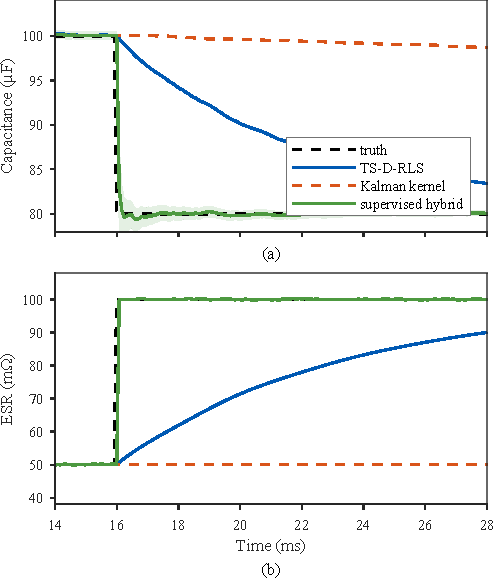
\includegraphics[width=\columnwidth]{fig_step_recovery.pdf}
\caption{Abrupt-step recovery on identical observation streams (seed 1):
(a) capacitance estimates after the $-20\%$ step; (b) ESR estimates after
the $2\times$ step. The shaded band is the supervised estimator's 95\%
interval, which widens at the reset and re-tightens. The Kalman kernel
freezes at the stale value; \TSRLS{} recovers over hundreds of cycles.}
\label{fig:recovery}
\end{figure}

\section{Conclusion}
A predeclared two-sided CUSUM supervisor over accepted and gate-rejected
normalized innovations, with a per-direction covariance reset, lets a
single topology-synchronous Kalman estimator keep calibrated steady-state
intervals while recovering from abrupt capacitor-health changes in a few
switching cycles and improving worst-case ramp tracking beyond both
published realizations, at about six extra operations per row. The
evidence is simulation-only and inherits the companion paper's plant and
observation boundaries; hardware validation, DCM operation, and
drift-aware interval inflation remain open.

\bibliographystyle{IEEEtran}
\bibliography{references}

\end{document}
